% ============================================================
% Day 14 - AI-Powered Analytics: Databricks Genie & Mosaic AI
% Databricks 14-Day AI Challenge
% Databricks Theme LaTeX Beamer Presentation
% ============================================================

\documentclass[aspectratio=169]{beamer}

% ============================================================
% Packages
% ============================================================
\usepackage{tikz}
\usepackage{graphicx}
\usepackage{hyperref}
\usepackage{xcolor}
\usepackage{amsmath}
\usepackage{amssymb}
\usepackage{booktabs}
\usepackage{listings}
\usepackage{fontspec}
\usepackage{array}
\usepackage{tabularx}
\usepackage{multirow}
\usepackage{colortbl}

\usetikzlibrary{shapes.geometric, arrows.meta, positioning, calc, fit, backgrounds, mindmap}

% ============================================================
% Databricks Color Palette
% ============================================================
\definecolor{databricksBlue}{RGB}{41, 49, 66}
\definecolor{databricksRed}{RGB}{220, 53, 69}
\definecolor{databricksYellow}{RGB}{255, 193, 7}
\definecolor{databricksGreen}{RGB}{76, 175, 80}
\definecolor{databricksGray}{RGB}{128, 128, 128}
\definecolor{databricksLightGray}{RGB}{245, 245, 245}
\definecolor{databricksWhite}{RGB}{255, 255, 255}
\definecolor{databricksOrange}{RGB}{255, 140, 0}
\definecolor{databricksPurple}{RGB}{156, 39, 176}
\definecolor{databricksCyan}{RGB}{0, 188, 212}

% ============================================================
% Beamer Theme Configuration
% ============================================================
\usetheme{default}
\usecolortheme{default}

% Set colors
\setbeamercolor{structure}{fg=databricksBlue}
\setbeamercolor{title}{fg=databricksWhite}
\setbeamercolor{subtitle}{fg=databricksLightGray}
\setbeamercolor{author}{fg=databricksWhite}
\setbeamercolor{date}{fg=databricksLightGray}
\setbeamercolor{frametitle}{fg=databricksWhite, bg=databricksBlue}
\setbeamercolor{normal text}{fg=databricksBlue}
\setbeamercolor{block title}{fg=databricksWhite, bg=databricksBlue}
\setbeamercolor{block body}{bg=databricksLightGray}
\setbeamercolor{itemize item}{fg=databricksBlue}
\setbeamercolor{itemize subitem}{fg=databricksRed}

% Set fonts
\setbeamerfont{title}{size=\Huge, series=\bfseries}
\setbeamerfont{subtitle}{size=\large}
\setbeamerfont{frametitle}{size=\Large, series=\bfseries}

% Remove navigation symbols
\setbeamertemplate{navigation symbols}{}

% ============================================================
% Custom Footer
% ============================================================
\setbeamertemplate{footline}{
    \leavevmode%
    \hbox{%
        \begin{beamercolorbox}[wd=.333333\paperwidth,ht=2.5ex,dp=1ex,left]{author in head/foot}%
            \usebeamerfont{author in head/foot}\hspace*{2ex}%
            \href{https://easy-ai-labs.lovable.app/}{\textcolor{databricksBlue}{Easy AI Labs}}
        \end{beamercolorbox}%
        \begin{beamercolorbox}[wd=.333333\paperwidth,ht=2.5ex,dp=1ex,center]{title in head/foot}%
            \usebeamerfont{title in head/foot}%
            \href{https://www.linkedin.com/in/yashkavaiya}{\textcolor{databricksBlue}{Yash Kavaiya}}
        \end{beamercolorbox}%
        \begin{beamercolorbox}[wd=.333333\paperwidth,ht=2.5ex,dp=1ex,right]{date in head/foot}%
            \usebeamerfont{date in head/foot}%
            \href{https://www.linkedin.com/company/genai-guru}{\textcolor{databricksBlue}{Gen AI Guru}}\hspace*{2ex}
            \textcolor{databricksGray}{\insertframenumber{} / \inserttotalframenumber}\hspace*{2ex}
        \end{beamercolorbox}%
    }%
    \vskip0pt%
}

% ============================================================
% Custom Header
% ============================================================
\setbeamertemplate{frametitle}{
    \nointerlineskip
    \begin{beamercolorbox}[wd=\paperwidth,ht=2.5ex,dp=1ex]{frametitle}
        \hspace*{1ex}\insertframetitle
    \end{beamercolorbox}
}

% ============================================================
% Code Listing Style
% ============================================================
\lstdefinestyle{pythonstyle}{
    language=Python,
    basicstyle=\ttfamily\footnotesize,
    keywordstyle=\color{databricksBlue}\bfseries,
    stringstyle=\color{databricksGreen},
    commentstyle=\color{databricksGray}\itshape,
    numberstyle=\tiny\color{databricksGray},
    numbers=left,
    numbersep=5pt,
    breaklines=true,
    showstringspaces=false,
    frame=single,
    rulecolor=\color{databricksBlue},
    backgroundcolor=\color{databricksLightGray},
    tabsize=2
}

\lstdefinestyle{sqlstyle}{
    language=SQL,
    basicstyle=\ttfamily\footnotesize,
    keywordstyle=\color{databricksBlue}\bfseries,
    stringstyle=\color{databricksGreen},
    commentstyle=\color{databricksGray}\itshape,
    numberstyle=\tiny\color{databricksGray},
    numbers=left,
    numbersep=5pt,
    breaklines=true,
    showstringspaces=false,
    frame=single,
    rulecolor=\color{databricksBlue},
    backgroundcolor=\color{databricksLightGray},
    tabsize=2
}

\lstset{style=pythonstyle}

% ============================================================
% Title Page Information
% ============================================================
\title{Day 14: AI-Powered Analytics}
\subtitle{Databricks Genie \& Mosaic AI}
\author{Yash Kavaiya}
\date{\today}

% ============================================================
% Document Begin
% ============================================================
\begin{document}

% ============================================================
% Title Slide
% ============================================================
{
\setbeamertemplate{footline}{}
\begin{frame}
\begin{tikzpicture}[remember picture, overlay]
    % Background
    \fill[databricksBlue] (current page.south west) rectangle (current page.north east);
    
    % Decorative elements
    \fill[databricksPurple, opacity=0.3] (current page.north west) ++(2,-2) circle (3.5cm);
    \fill[databricksCyan, opacity=0.2] (current page.south east) ++(-2,2) circle (4cm);
    \fill[databricksYellow, opacity=0.2] (current page.east) ++(-3,1) circle (2.5cm);
    \fill[databricksGreen, opacity=0.15] (current page.west) ++(3,-1) circle (2cm);
    
    % Title content
    \node[anchor=center, text width=0.85\paperwidth, align=center] at (current page.center) {
        {\Huge\bfseries\textcolor{databricksWhite}{Day 14}}\\[0.3cm]
        {\LARGE\textcolor{databricksYellow}{AI-Powered Analytics}}\\[0.2cm]
        {\large\textcolor{databricksCyan}{Databricks Genie \& Mosaic AI}}\\[0.8cm]
        {\normalsize\textcolor{databricksLightGray}{Databricks 14-Day AI Challenge}}\\[0.5cm]
        {\normalsize\textcolor{databricksWhite}{Yash Kavaiya}}
    };
    
    % Bottom decoration
    \fill[databricksCyan] (current page.south west) rectangle ++(0.33\paperwidth, 0.15);
    \fill[databricksPurple] (current page.south west) ++(0.33\paperwidth,0) rectangle ++(0.34\paperwidth, 0.15);
    \fill[databricksYellow] (current page.south west) ++(0.67\paperwidth,0) rectangle ++(0.33\paperwidth, 0.15);
\end{tikzpicture}
\end{frame}
}

% ============================================================
% Agenda Slide
% ============================================================
\begin{frame}{Agenda}
    \begin{columns}[T]
        \begin{column}{0.48\textwidth}
            \textcolor{databricksBlue}{$\bullet$} \textcolor{databricksBlue}{\textbf{AI-Powered Analytics}}
            \begin{itemize}
                \item[\textcolor{databricksRed}{$\triangleright$}] What it is and why it matters
                \item[\textcolor{databricksRed}{$\triangleright$}] Traditional vs AI workflows
            \end{itemize}
            \vspace{0.3cm}
            
            \textcolor{databricksBlue}{$\bullet$} \textcolor{databricksBlue}{\textbf{Databricks Genie}}
            \begin{itemize}
                \item[\textcolor{databricksRed}{$\triangleright$}] Natural Language to SQL
                \item[\textcolor{databricksRed}{$\triangleright$}] Genie Data Spaces
            \end{itemize}
            \vspace{0.3cm}
            
            \textcolor{databricksBlue}{$\bullet$} \textcolor{databricksBlue}{\textbf{Mosaic AI Platform}}
            \begin{itemize}
                \item[\textcolor{databricksRed}{$\triangleright$}] Foundation Models
                \item[\textcolor{databricksRed}{$\triangleright$}] Model Serving \& Vector Search
            \end{itemize}
        \end{column}
        
        \begin{column}{0.48\textwidth}
            \textcolor{databricksBlue}{$\bullet$} \textcolor{databricksBlue}{\textbf{Generative AI Integration}}
            \begin{itemize}
                \item[\textcolor{databricksRed}{$\triangleright$}] AI Functions in SQL
                \item[\textcolor{databricksRed}{$\triangleright$}] RAG Applications
            \end{itemize}
            \vspace{0.3cm}
            
            \textcolor{databricksBlue}{$\bullet$} \textcolor{databricksBlue}{\textbf{AI-Assisted Analysis}}
            \begin{itemize}
                \item[\textcolor{databricksRed}{$\triangleright$}] Sentiment Analysis
                \item[\textcolor{databricksRed}{$\triangleright$}] Automated Insights
            \end{itemize}
            \vspace{0.3cm}
            
            \textcolor{databricksBlue}{$\bullet$} \textcolor{databricksBlue}{\textbf{Best Practices}}
            \begin{itemize}
                \item[\textcolor{databricksRed}{$\triangleright$}] Data quality and governance
                \item[\textcolor{databricksRed}{$\triangleright$}] Cost optimization
            \end{itemize}
        \end{column}
    \end{columns}
\end{frame}

% ============================================================
% Section: What is AI-Powered Analytics
% ============================================================
\begin{frame}{What is AI-Powered Analytics?}
    \begin{block}{Definition}
        The convergence of AI and traditional data analytics — enabling natural language interactions, intelligent recommendations, and automated analytical tasks.
    \end{block}
    
    \vspace{0.3cm}
    
    \begin{columns}[T]
        \begin{column}{0.48\textwidth}
            \textcolor{databricksBlue}{\textbf{Business Value:}}
            \begin{itemize}
                \item[\textcolor{databricksBlue}{$\bullet$}] Question to insight: hours → seconds
                \item[\textcolor{databricksBlue}{$\bullet$}] Empowers non-technical users
                \item[\textcolor{databricksBlue}{$\bullet$}] Data democratization
                \item[\textcolor{databricksBlue}{$\bullet$}] Faster decision-making
            \end{itemize}
        \end{column}
        
        \begin{column}{0.48\textwidth}
            \textcolor{databricksRed}{\textbf{Technical Benefits:}}
            \begin{itemize}
                \item[\textcolor{databricksRed}{$\triangleright$}] Automatic query optimization
                \item[\textcolor{databricksRed}{$\triangleright$}] Intelligent data discovery
                \item[\textcolor{databricksRed}{$\triangleright$}] Pattern recognition at scale
                \item[\textcolor{databricksRed}{$\triangleright$}] Predictive insights generation
            \end{itemize}
        \end{column}
    \end{columns}
\end{frame}

% ============================================================
% Section: Traditional vs AI Workflow
% ============================================================
\begin{frame}{Traditional vs AI-Powered Analytics}
    \centering
    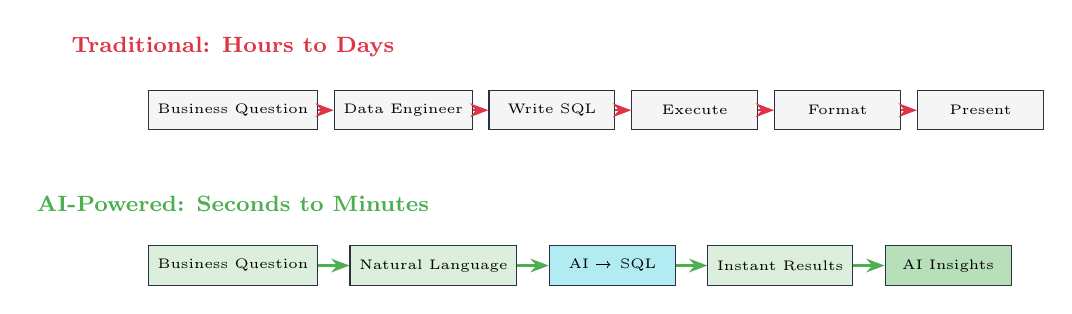
\begin{tikzpicture}[
        node distance=0.4cm,
        box/.style={rectangle, draw=databricksBlue, fill=databricksLightGray, minimum width=1.6cm, minimum height=0.5cm, align=center, font=\tiny},
        arrow/.style={-Stealth, thick, databricksBlue}
    ]
        % Traditional workflow
        \node[font=\footnotesize\bfseries, text=databricksRed] (t1) at (-4, 2) {Traditional: Hours to Days};
        \node[box, below=0.3cm of t1] (ta) {Business Question};
        \node[box, right=0.2cm of ta] (tb) {Data Engineer};
        \node[box, right=0.2cm of tb] (tc) {Write SQL};
        \node[box, right=0.2cm of tc] (td) {Execute};
        \node[box, right=0.2cm of td] (te) {Format};
        \node[box, right=0.2cm of te] (tf) {Present};
        
        \draw[arrow, databricksRed] (ta) -- (tb);
        \draw[arrow, databricksRed] (tb) -- (tc);
        \draw[arrow, databricksRed] (tc) -- (td);
        \draw[arrow, databricksRed] (td) -- (te);
        \draw[arrow, databricksRed] (te) -- (tf);
        
        % AI-Powered workflow
        \node[font=\footnotesize\bfseries, text=databricksGreen] (a1) at (-4, 0) {AI-Powered: Seconds to Minutes};
        \node[box, fill=databricksGreen!20, below=0.3cm of a1] (aa) {Business Question};
        \node[box, fill=databricksGreen!20, right=0.4cm of aa] (ab) {Natural Language};
        \node[box, fill=databricksCyan!30, right=0.4cm of ab] (ac) {AI → SQL};
        \node[box, fill=databricksGreen!20, right=0.4cm of ac] (ad) {Instant Results};
        \node[box, fill=databricksGreen!40, right=0.4cm of ad] (ae) {AI Insights};
        
        \draw[arrow, databricksGreen] (aa) -- (ab);
        \draw[arrow, databricksGreen] (ab) -- (ac);
        \draw[arrow, databricksGreen] (ac) -- (ad);
        \draw[arrow, databricksGreen] (ad) -- (ae);
    \end{tikzpicture}
    
    \vspace{0.5cm}
    
    
\begin{tikzpicture}
        \node[draw=databricksBlue, fill=databricksLightGray, rounded corners, text width=11cm, align=center, inner sep=8pt] {
            \textcolor{databricksBlue}{\textbf{Key Insight:}} AI-powered analytics compresses multi-step workflows into streamlined, accessible processes!
        };
    \end{tikzpicture}
\end{frame}

% ============================================================
% Section: Databricks Genie
% ============================================================
\begin{frame}{Databricks Genie: Natural Language to SQL}
    \begin{block}{What is Genie?}
        An AI-powered conversational interface that transforms natural language questions into SQL queries — like having a 24/7 data analyst!
    \end{block}
    
    \vspace{0.3cm}
    
    \centering
    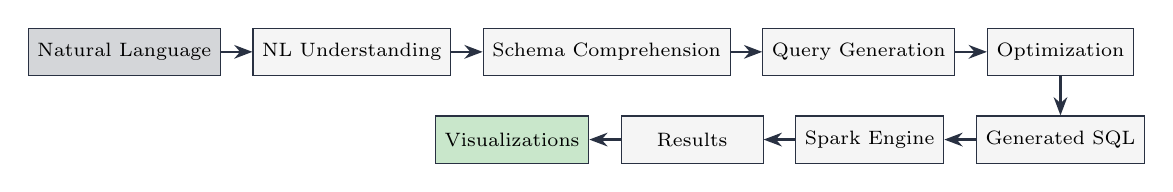
\begin{tikzpicture}[
        node distance=0.5cm,
        box/.style={rectangle, draw=databricksBlue, fill=databricksLightGray, minimum width=1.8cm, minimum height=0.6cm, align=center, font=\scriptsize},
        arrow/.style={-Stealth, thick, databricksBlue}
    ]
        % Input
        \node[box, fill=databricksBlue!20] (nl) {Natural Language};
        
        % Processing
        \node[box, right=0.4cm of nl] (nlu) {NL Understanding};
        \node[box, right=0.4cm of nlu] (sc) {Schema Comprehension};
        \node[box, right=0.4cm of sc] (qg) {Query Generation};
        \node[box, right=0.4cm of qg] (opt) {Optimization};
        
        % Output
        \node[box, below=0.5cm of opt] (sql) {Generated SQL};
        \node[box, left=0.4cm of sql] (eng) {Spark Engine};
        \node[box, left=0.4cm of eng] (res) {Results};
        \node[box, fill=databricksGreen!30, left=0.4cm of res] (viz) {Visualizations};
        
        \draw[arrow] (nl) -- (nlu);
        \draw[arrow] (nlu) -- (sc);
        \draw[arrow] (sc) -- (qg);
        \draw[arrow] (qg) -- (opt);
        \draw[arrow] (opt) -- (sql);
        \draw[arrow] (sql) -- (eng);
        \draw[arrow] (eng) -- (res);
        \draw[arrow] (res) -- (viz);
    \end{tikzpicture}
\end{frame}

% ============================================================
% Section: Genie Data Spaces
% ============================================================
\begin{frame}{Genie Data Spaces}
    \begin{block}{What is a Data Space?}
        A curated environment defining the scope of data Genie can access — a focused "sandbox" for specific business domains.
    \end{block}
    
    \vspace{0.3cm}
    
    \centering
    \small
    \begin{tabular}{l c c}
        \toprule
        \textbf{Aspect} & \textbf{Without Data Spaces} & \textbf{With Data Spaces} \\
        \midrule
        \rowcolor{databricksLightGray}
        Scope & Access to all tables & Focused on relevant data \\
        Accuracy & May query wrong tables & Precise table selection \\
        \rowcolor{databricksLightGray}
        Security & Broad access concerns & Controlled exposure \\
        Performance & Searches entire catalog & Faster comprehension \\
        \rowcolor{databricksLightGray}
        Context & Generic understanding & Domain-specific knowledge \\
        \bottomrule
    \end{tabular}
\end{frame}

% ============================================================
% Section: Genie Query Examples
% ============================================================
\begin{frame}{Genie Query Examples}
    \begin{columns}[T]
        \begin{column}{0.48\textwidth}
            \textcolor{databricksBlue}{\textbf{"Total revenue by category"}}
            \begin{itemize}
                \item[\textcolor{databricksRed}{$\triangleright$}] "total revenue" → SUM aggregation
                \item[\textcolor{databricksRed}{$\triangleright$}] "by category" → GROUP BY
            \end{itemize}
            
            \vspace{0.3cm}
            
            \textcolor{databricksGreen}{\textbf{"Highest conversion rate?"}}
            \begin{itemize}
                \item[\textcolor{databricksRed}{$\triangleright$}] Conversion = Purchases/Views
                \item[\textcolor{databricksRed}{$\triangleright$}] ORDER BY DESC + LIMIT
            \end{itemize}
            
            \vspace{0.2cm}
            $$\text{Conv Rate} = \frac{\text{Purchases}}{\text{Views}} \times 100$$
        \end{column}
        
        \begin{column}{0.48\textwidth}
            \textcolor{databricksOrange}{\textbf{"Daily purchases trend?"}}
            \begin{itemize}
                \item[\textcolor{databricksRed}{$\triangleright$}] Time series analysis
                \item[\textcolor{databricksRed}{$\triangleright$}] COUNT by DATE
            \end{itemize}
            
            \vspace{0.3cm}
            
            \textcolor{databricksPurple}{\textbf{"Viewed but never purchased?"}}
            \begin{itemize}
                \item[\textcolor{databricksRed}{$\triangleright$}] LEFT JOIN with NULL check
                \item[\textcolor{databricksRed}{$\triangleright$}] Remarketing opportunities!
            \end{itemize}
        \end{column}
    \end{columns}
\end{frame}

% ============================================================
% Section: Mosaic AI Platform
% ============================================================
\begin{frame}{Mosaic AI Platform}
    \begin{block}{What is Mosaic AI?}
        Databricks' comprehensive AI/ML platform for training, deploying, and managing AI models at enterprise scale.
    \end{block}
    
    \vspace{0.2cm}
    
    \centering
    
\begin{tikzpicture}[
        node distance=0.3cm,
        comp/.style={rectangle, draw=databricksBlue, fill=databricksLightGray, minimum width=2cm, minimum height=0.6cm, align=center, font=\scriptsize, rounded corners}
    ]
        % Main components
        \node[comp, fill=databricksBlue, text=white] (fm) {Foundation Models};
        \node[comp, fill=databricksRed, text=white, right=0.3cm of fm] (ms) {Model Serving};
        \node[comp, fill=databricksGreen, text=white, right=0.3cm of ms] (vs) {Vector Search};
        \node[comp, fill=databricksPurple, text=white, right=0.3cm of vs] (ag) {AI Agents};
        \node[comp, fill=databricksOrange, text=white, right=0.3cm of ag] (ml) {MLflow};
        
        % Sub-labels
        \node[font=\tiny, below=0.1cm of fm] {DBRX, Llama, External};
        \node[font=\tiny, below=0.1cm of ms] {REST APIs, Auto-scale};
        \node[font=\tiny, below=0.1cm of vs] {Semantic Search, RAG};
        \node[font=\tiny, below=0.1cm of ag] {Multi-step reasoning};
        \node[font=\tiny, below=0.1cm of ml] {Track, Registry, Deploy};
    \end{tikzpicture}
    
    \vspace{0.3cm}
    
    \begin{columns}[T]
        \begin{column}{0.32\textwidth}
            \centering
            \textcolor{databricksBlue}{\textbf{Training}}\\
            \footnotesize Fine-tuning \& Pre-training
        \end{column}
        \begin{column}{0.32\textwidth}
            \centering
            \textcolor{databricksRed}{\textbf{Serving}}\\
            \footnotesize Real-time, Batch, Streaming
        \end{column}
        \begin{column}{0.32\textwidth}
            \centering
            \textcolor{databricksGreen}{\textbf{Tools}}\\
            \footnotesize Feature Store, Evaluation
        \end{column}
    \end{columns}
\end{frame}

% ============================================================
% Section: Foundation Model APIs
% ============================================================
\begin{frame}{Foundation Model APIs}
    \begin{columns}[T]
        \begin{column}{0.48\textwidth}
            \textcolor{databricksBlue}{\textbf{Available Models:}}
            \begin{itemize}
                \item[\textcolor{databricksBlue}{$\bullet$}] \textbf{DBRX} — Databricks' own LLM
                \begin{itemize}
                    \item[\textcolor{databricksRed}{$\triangleright$}] Optimized for enterprise
                \end{itemize}
                \item[\textcolor{databricksBlue}{$\bullet$}] \textbf{Llama Models} — Meta's open-source
                \begin{itemize}
                    \item[\textcolor{databricksRed}{$\triangleright$}] Various sizes available
                \end{itemize}
                \item[\textcolor{databricksBlue}{$\bullet$}] \textbf{External Models} — AI Gateway
                \begin{itemize}
                    \item[\textcolor{databricksRed}{$\triangleright$}] OpenAI, Anthropic, etc.
                \end{itemize}
            \end{itemize}
        \end{column}
        
        \begin{column}{0.48\textwidth}
            \textcolor{databricksGreen}{\textbf{Key Benefits:}}
            \begin{itemize}
                \item[\textcolor{databricksGreen}{$\checkmark$}] No infrastructure management
                \item[\textcolor{databricksGreen}{$\checkmark$}] Pay-per-use pricing
                \item[\textcolor{databricksGreen}{$\checkmark$}] Unified API interface
                \item[\textcolor{databricksGreen}{$\checkmark$}] Built-in governance
                \item[\textcolor{databricksGreen}{$\checkmark$}] Enterprise security
            \end{itemize}
        \end{column}
    \end{columns}
\end{frame}

% ============================================================
% Section: Model Serving Types
% ============================================================
\begin{frame}{Model Serving Types}
    \centering
    \begin{tabular}{l c c c}
        \toprule
        \textbf{Serving Type} & \textbf{Use Case} & \textbf{Latency} & \textbf{Scaling} \\
        \midrule
        \rowcolor{databricksLightGray}
        \textcolor{databricksBlue}{\textbf{Real-time}} & Interactive apps & < 100ms & Auto-scale \\
        \textcolor{databricksRed}{\textbf{Batch}} & Large-scale scoring & Minutes & Parallel jobs \\
        \rowcolor{databricksLightGray}
        \textcolor{databricksGreen}{\textbf{Streaming}} & Continuous predictions & Seconds & Event-driven \\
        \bottomrule
    \end{tabular}
    
    \vspace{0.5cm}
    
    
\begin{tikzpicture}
        \node[draw=databricksBlue, fill=databricksLightGray, rounded corners, text width=11cm, align=center, inner sep=8pt] {
            \textcolor{databricksBlue}{\textbf{Tip:}} Use \texttt{scale\_to\_zero\_enabled=True} to minimize costs when endpoints are idle!
        };
    \end{tikzpicture}
\end{frame}

% ============================================================
% Section: Vector Search
% ============================================================
\begin{frame}{Vector Search for Semantic Retrieval}
    \begin{block}{What is Vector Search?}
        Enables semantic search by storing and querying high-dimensional vector embeddings — essential for RAG applications!
    \end{block}
    
    \vspace{0.2cm}
    
    \begin{columns}[T]
        \begin{column}{0.48\textwidth}
            \textcolor{databricksBlue}{\textbf{How it Works:}}
            \begin{itemize}
                \item[\textcolor{databricksBlue}{$\bullet$}] Text → Embeddings (vectors)
                \item[\textcolor{databricksBlue}{$\bullet$}] Similar items = close vectors
                \item[\textcolor{databricksBlue}{$\bullet$}] Query by similarity, not keywords
            \end{itemize}
            
            \vspace{0.3cm}
            
            \textcolor{databricksGreen}{\textbf{Cosine Similarity:}}
            $$\cos(\theta) = \frac{A \cdot B}{\|A\| \|B\|}$$
        \end{column}
        
        \begin{column}{0.48\textwidth}
            \centering
            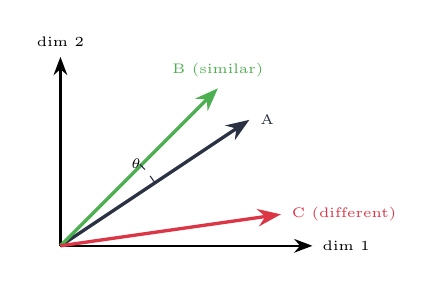
\begin{tikzpicture}[scale=0.8]
                % Axes
                \draw[-Stealth, thick] (0,0) -- (4,0) node[right] {\tiny dim 1};
                \draw[-Stealth, thick] (0,0) -- (0,3) node[above] {\tiny dim 2};
                
                % Vectors
                \draw[-Stealth, very thick, databricksBlue] (0,0) -- (3,2) node[right] {\tiny A};
                \draw[-Stealth, very thick, databricksGreen] (0,0) -- (2.5,2.5) node[above] {\tiny B (similar)};
                \draw[-Stealth, very thick, databricksRed] (0,0) -- (3.5,0.5) node[right] {\tiny C (different)};
                
                % Angle
                \draw[databricksBlue, dashed] (1.5,1) arc (33:45:1.8);
                \node at (1.2,1.3) {\tiny $\theta$};
            \end{tikzpicture}
            
            \vspace{0.2cm}
            \footnotesize Range: $-1$ to $1$ (1 = identical)
        \end{column}
    \end{columns}
\end{frame}

% ============================================================
% Section: AI Agents
% ============================================================
\begin{frame}{AI Agents: Autonomous AI Systems}
    \centering
    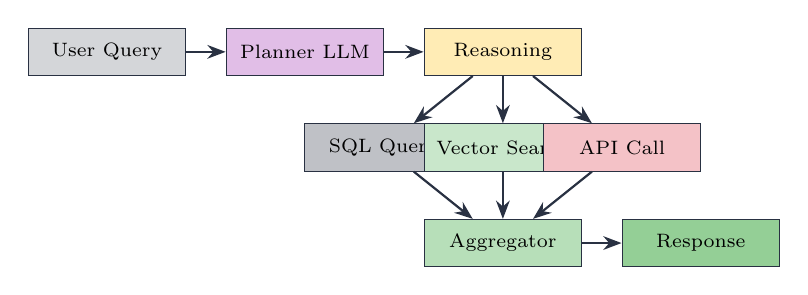
\begin{tikzpicture}[
        node distance=0.5cm,
        box/.style={rectangle, draw=databricksBlue, fill=databricksLightGray, minimum width=2cm, minimum height=0.6cm, align=center, font=\scriptsize},
        arrow/.style={-Stealth, thick, databricksBlue}
    ]
        % Agent flow
        \node[box, fill=databricksBlue!20] (query) {User Query};
        \node[box, fill=databricksPurple!30, right=0.5cm of query] (planner) {Planner LLM};
        \node[box, fill=databricksYellow!30, right=0.5cm of planner] (reason) {Reasoning};
        
        % Tools
        \node[box, fill=databricksBlue!30, below left=0.6cm and -0.5cm of reason] (t1) {SQL Query};
        \node[box, fill=databricksGreen!30, below=0.6cm of reason] (t2) {Vector Search};
        \node[box, fill=databricksRed!30, below right=0.6cm and -0.5cm of reason] (t3) {API Call};
        
        % Output
        \node[box, fill=databricksGreen!40, below=0.6cm of t2] (agg) {Aggregator};
        \node[box, fill=databricksGreen!60, right=0.5cm of agg] (resp) {Response};
        
        \draw[arrow] (query) -- (planner);
        \draw[arrow] (planner) -- (reason);
        \draw[arrow] (reason) -- (t1);
        \draw[arrow] (reason) -- (t2);
        \draw[arrow] (reason) -- (t3);
        \draw[arrow] (t1) -- (agg);
        \draw[arrow] (t2) -- (agg);
        \draw[arrow] (t3) -- (agg);
        \draw[arrow] (agg) -- (resp);
    \end{tikzpicture}
    
    \vspace{0.4cm}
    
    \begin{columns}[T]
        \begin{column}{0.48\textwidth}
            \textcolor{databricksBlue}{\textbf{Capabilities:}}
            \begin{itemize}
                \item[\textcolor{databricksBlue}{$\bullet$}] Multi-step reasoning
                \item[\textcolor{databricksBlue}{$\bullet$}] Tool use (SQL, APIs)
            \end{itemize}
        \end{column}
        \begin{column}{0.48\textwidth}
            \begin{itemize}
                \item[\textcolor{databricksBlue}{$\bullet$}] Memory management
                \item[\textcolor{databricksBlue}{$\bullet$}] Self-correction
            \end{itemize}
        \end{column}
    \end{columns}
\end{frame}

% ============================================================
% Section: AI Functions in SQL
% ============================================================
\begin{frame}{AI Functions in Databricks SQL}
    \centering
    \small
    \begin{tabular}{l l l}
        \toprule
        \textbf{Function} & \textbf{Description} & \textbf{Use Case} \\
        \midrule
        \rowcolor{databricksLightGray}
        \texttt{ai\_analyze\_sentiment()} & Detect +/- sentiment & Feedback analysis \\
        \texttt{ai\_extract\_entities()} & Extract named entities & Info extraction \\
        \rowcolor{databricksLightGray}
        \texttt{ai\_summarize()} & Generate summaries & Document processing \\
        \texttt{ai\_classify()} & Categorize text & Ticket routing \\
        \rowcolor{databricksLightGray}
        \texttt{ai\_translate()} & Language translation & Globalization \\
        \texttt{ai\_query()} & Custom LLM queries & Flexible AI tasks \\
        \bottomrule
    \end{tabular}
    
    \vspace{0.4cm}
    
    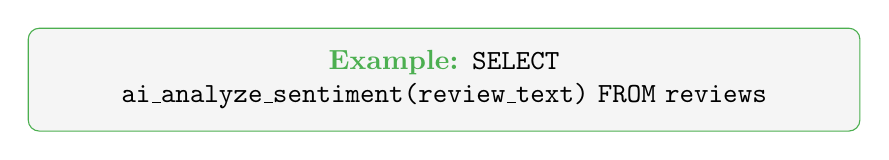
\begin{tikzpicture}
        \node[draw=databricksGreen, fill=databricksLightGray, rounded corners, text width=10cm, align=center, inner sep=8pt] {
            \textcolor{databricksGreen}{\textbf{Example:}} \texttt{SELECT ai\_analyze\_sentiment(review\_text) FROM reviews}
        };
    \end{tikzpicture}
\end{frame}

% ============================================================
% Section: RAG Architecture
% ============================================================
\begin{frame}{RAG: Retrieval-Augmented Generation}
    \centering
    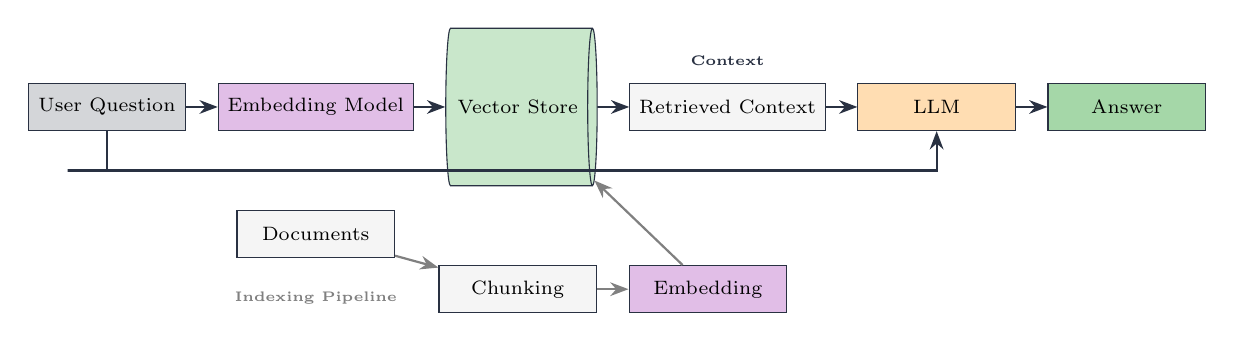
\begin{tikzpicture}[
        node distance=0.4cm,
        box/.style={rectangle, draw=databricksBlue, fill=databricksLightGray, minimum width=2cm, minimum height=0.6cm, align=center, font=\scriptsize},
        arrow/.style={-Stealth, thick, databricksBlue}
    ]
        % Query path
        \node[box, fill=databricksBlue!20] (q) {User Question};
        \node[box, fill=databricksPurple!30, right=0.4cm of q] (em) {Embedding Model};
        \node[box, fill=databricksGreen!30, right=0.4cm of em, shape=cylinder, aspect=0.3] (vs) {Vector Store};
        \node[box, right=0.4cm of vs] (ctx) {Retrieved Context};
        \node[box, fill=databricksOrange!30, right=0.4cm of ctx] (llm) {LLM};
        \node[box, fill=databricksGreen!50, right=0.4cm of llm] (ans) {Answer};
        
        % Document path (below)
        \node[box, fill=databricksLightGray, below=1cm of em] (docs) {Documents};
        \node[box, below=1cm of vs] (chunk) {Chunking};
        \node[box, fill=databricksPurple!30, right=0.4cm of chunk] (emb) {Embedding};
        
        \draw[arrow] (q) -- (em);
        \draw[arrow] (em) -- (vs);
        \draw[arrow] (vs) -- (ctx);
        \draw[arrow] (ctx) -- (llm);
        \draw[arrow] (q.south) |- ++(-0.5,-0.5) -| (llm.south);
        \draw[arrow] (llm) -- (ans);
        
        \draw[arrow, databricksGray] (docs) -- (chunk);
        \draw[arrow, databricksGray] (chunk) -- (emb);
        \draw[arrow, databricksGray] (emb) -- (vs);
        
        % Labels
        \node[font=\tiny\bfseries, text=databricksBlue, above=0.1cm of ctx] {Context};
        \node[font=\tiny\bfseries, text=databricksGray, below=0.3cm of docs] {Indexing Pipeline};
    \end{tikzpicture}
    
    \vspace{0.3cm}
    
    \begin{columns}[T]
        \begin{column}{0.48\textwidth}
            \textcolor{databricksBlue}{\textbf{How RAG Works:}}
            \begin{itemize}
                \item[\textcolor{databricksBlue}{1.}] Embed user question
                \item[\textcolor{databricksBlue}{2.}] Search for relevant docs
            \end{itemize}
        \end{column}
        \begin{column}{0.48\textwidth}
            \begin{itemize}
                \item[\textcolor{databricksBlue}{3.}] Provide context to LLM
                \item[\textcolor{databricksBlue}{4.}] Generate grounded answer
            \end{itemize}
        \end{column}
    \end{columns}
\end{frame}

% ============================================================
% Section: Sentiment Analysis
% ============================================================
\begin{frame}{Sentiment Analysis Implementation}
    \begin{columns}[T]
        \begin{column}{0.48\textwidth}
            \textcolor{databricksBlue}{\textbf{How it Works:}}
            \begin{itemize}
                \item[\textcolor{databricksBlue}{$\bullet$}] Text → Model → Label + Score
                \item[\textcolor{databricksBlue}{$\bullet$}] POSITIVE / NEGATIVE
                \item[\textcolor{databricksBlue}{$\bullet$}] Confidence 0-100\%
            \end{itemize}
            
            \vspace{0.3cm}
            
            \textcolor{databricksGreen}{\textbf{Confidence Score (Softmax):}}
            $$P(\text{sent}|\text{text}) = \frac{e^{z_i}}{\sum_j e^{z_j}}$$
        \end{column}
        
        \begin{column}{0.48\textwidth}
            \textcolor{databricksRed}{\textbf{Use Cases:}}
            \begin{itemize}
                \item[\textcolor{databricksRed}{$\triangleright$}] Product review analysis
                \item[\textcolor{databricksRed}{$\triangleright$}] Customer feedback
                \item[\textcolor{databricksRed}{$\triangleright$}] Social media monitoring
                \item[\textcolor{databricksRed}{$\triangleright$}] Support ticket triage
            \end{itemize}
            
            \vspace{0.3cm}
            
            \footnotesize
            \textcolor{databricksGreen}{$\checkmark$} "Amazing product!" → POSITIVE\\
            \textcolor{databricksRed}{$\times$} "Terrible quality" → NEGATIVE
        \end{column}
    \end{columns}
\end{frame}

% ============================================================
% Section: AI-Assisted Analysis Capabilities
% ============================================================
\begin{frame}{AI-Assisted Analysis}
    \begin{block}{Definition}
        Augments human analytical capabilities with AI tools that automatically detect patterns, generate hypotheses, and provide explanations.
    \end{block}
    
    \vspace{0.3cm}
    
    \begin{columns}[T]
        \begin{column}{0.48\textwidth}
            
\begin{tikzpicture}
                \node[fill=databricksBlue, text=white, rounded corners, minimum width=4cm, minimum height=0.6cm, font=\footnotesize\bfseries] at (0,0) {Anomaly Detection};
            \end{tikzpicture}
            \footnotesize Identify unusual patterns automatically
            
            \vspace{0.3cm}
            
            
\begin{tikzpicture}
                \node[fill=databricksRed, text=white, rounded corners, minimum width=4cm, minimum height=0.6cm, font=\footnotesize\bfseries] at (0,0) {Root Cause Analysis};
            \end{tikzpicture}
            \footnotesize Trace back factors causing changes
        \end{column}
        
        \begin{column}{0.48\textwidth}
            
\begin{tikzpicture}
                \node[fill=databricksGreen, text=white, rounded corners, minimum width=4cm, minimum height=0.6cm, font=\footnotesize\bfseries] at (0,0) {Predictive Insights};
            \end{tikzpicture}
            \footnotesize Forecast future trends
            
            \vspace{0.3cm}
            
            
\begin{tikzpicture}
                \node[fill=databricksPurple, text=white, rounded corners, minimum width=4cm, minimum height=0.6cm, font=\footnotesize\bfseries] at (0,0) {NL Explanations};
            \end{tikzpicture}
            \footnotesize Convert findings to plain English
        \end{column}
    \end{columns}
\end{frame}

% ============================================================
% Section: Best Practices - Data Quality
% ============================================================
\begin{frame}{Best Practices: Data Quality}
    \centering
    \small
    \begin{tabular}{l l l}
        \toprule
        \textbf{Issue} & \textbf{Impact on AI} & \textbf{Solution} \\
        \midrule
        \rowcolor{databricksLightGray}
        Missing values & Incomplete analysis & Imputation or filtering \\
        Inconsistent formats & Parsing errors & Standardization \\
        \rowcolor{databricksLightGray}
        Duplicate records & Inflated metrics & Deduplication \\
        Outdated data & Irrelevant insights & Regular refresh \\
        \rowcolor{databricksLightGray}
        Biased samples & Skewed predictions & Stratified sampling \\
        \bottomrule
    \end{tabular}
    
    \vspace{0.4cm}
    
    
\begin{tikzpicture}
        \node[draw=databricksRed, fill=databricksLightGray, rounded corners, text width=10cm, align=center, inner sep=8pt] {
            \textcolor{databricksRed}{\textbf{Remember:}} AI systems are only as good as the data they analyze!
        };
    \end{tikzpicture}
\end{frame}

% ============================================================
% Section: Prompt Engineering
% ============================================================
\begin{frame}{Prompt Engineering for Better Results}
    \centering
    \small
    \begin{tabular}{l l}
        \toprule
        \textbf{Less Effective} & \textbf{More Effective} \\
        \midrule
        \rowcolor{databricksLightGray}
        "Show me data" & "Show monthly revenue by category for Q4 2024" \\
        "Sales info" & "Total sales amount grouped by customer segment" \\
        \rowcolor{databricksLightGray}
        "Best products" & "Top 10 products with highest profit margin" \\
        \bottomrule
    \end{tabular}
    
    \vspace{0.4cm}
    
    \begin{columns}[T]
        \begin{column}{0.48\textwidth}
            \textcolor{databricksBlue}{\textbf{LLM Prompt Tips:}}
            \begin{itemize}
                \item[\textcolor{databricksBlue}{1.}] Be Specific
                \item[\textcolor{databricksBlue}{2.}] Provide Context
                \item[\textcolor{databricksBlue}{3.}] Specify Format
            \end{itemize}
        \end{column}
        \begin{column}{0.48\textwidth}
            \begin{itemize}
                \item[\textcolor{databricksBlue}{4.}] Use Examples
                \item[\textcolor{databricksBlue}{5.}] Set Boundaries
            \end{itemize}
        \end{column}
    \end{columns}
\end{frame}

% ============================================================
% Section: Cost Optimization
% ============================================================
\begin{frame}{Cost Optimization Strategies}
    \centering
    \begin{tabular}{l l c}
        \toprule
        \textbf{Strategy} & \textbf{Description} & \textbf{Savings} \\
        \midrule
        \rowcolor{databricksLightGray}
        \textcolor{databricksBlue}{\textbf{Right-sizing}} & Match compute to workload & 20-40\% \\
        \textcolor{databricksGreen}{\textbf{Caching}} & Store frequent query results & 30-50\% \\
        \rowcolor{databricksLightGray}
        \textcolor{databricksOrange}{\textbf{Batch Processing}} & Combine small requests & 15-25\% \\
        \textcolor{databricksPurple}{\textbf{Model Selection}} & Use smaller models when appropriate & 40-60\% \\
        \bottomrule
    \end{tabular}
    
    \vspace{0.4cm}
    
    
\begin{tikzpicture}
        \node[draw=databricksGreen, fill=databricksLightGray, rounded corners, text width=10cm, align=center, inner sep=8pt] {
            \textcolor{databricksGreen}{\textbf{Pro Tip:}} Start with foundation models, fine-tune only when needed!
        };
    \end{tikzpicture}
\end{frame}

% ============================================================
% Section: When to Use What
% ============================================================
\begin{frame}{Quick Reference: When to Use What}
    \centering
    \begin{tabular}{l l}
        \toprule
        \textbf{Need} & \textbf{Solution} \\
        \midrule
        \rowcolor{databricksLightGray}
        Business users need self-service analytics & \textcolor{databricksBlue}{Databricks Genie} \\
        Deploy custom ML models as APIs & \textcolor{databricksRed}{Mosaic AI Model Serving} \\
        \rowcolor{databricksLightGray}
        Build semantic search or Q\&A systems & \textcolor{databricksGreen}{Vector Search + RAG} \\
        Analyze text data (sentiment, classification) & \textcolor{databricksPurple}{Foundation Model APIs} \\
        \rowcolor{databricksLightGray}
        Track experiments and model versions & \textcolor{databricksOrange}{MLflow} \\
        Create automated insights & \textcolor{databricksCyan}{AI Functions + Custom Analysis} \\
        \bottomrule
    \end{tabular}
\end{frame}

% ============================================================
% Section: Key Takeaways
% ============================================================
\begin{frame}{Key Takeaways}
    \begin{columns}[T]
        \begin{column}{0.48\textwidth}
            
\begin{tikzpicture}
                \node[fill=databricksBlue, text=white, rounded corners, minimum width=4.5cm, minimum height=0.6cm, font=\footnotesize\bfseries] at (0,0) {1. Databricks Genie};
            \end{tikzpicture}
            \footnotesize NL to SQL — democratize data access
            
            \vspace{0.2cm}
            
            
\begin{tikzpicture}
                \node[fill=databricksRed, text=white, rounded corners, minimum width=4.5cm, minimum height=0.6cm, font=\footnotesize\bfseries] at (0,0) {2. Mosaic AI};
            \end{tikzpicture}
            \footnotesize Comprehensive AI/ML platform
            
            \vspace{0.2cm}
            
            
\begin{tikzpicture}
                \node[fill=databricksGreen, text=white, rounded corners, minimum width=4.5cm, minimum height=0.6cm, font=\footnotesize\bfseries] at (0,0) {3. Foundation Models};
            \end{tikzpicture}
            \footnotesize No infrastructure management
        \end{column}
        
        \begin{column}{0.48\textwidth}
            
\begin{tikzpicture}
                \node[fill=databricksPurple, text=white, rounded corners, minimum width=4.5cm, minimum height=0.6cm, font=\footnotesize\bfseries] at (0,0) {4. Vector Search};
            \end{tikzpicture}
            \footnotesize Essential for RAG applications
            
            \vspace{0.2cm}
            
            
\begin{tikzpicture}
                \node[fill=databricksOrange, text=white, rounded corners, minimum width=4.5cm, minimum height=0.6cm, font=\footnotesize\bfseries] at (0,0) {5. AI-Assisted Analysis};
            \end{tikzpicture}
            \footnotesize Amplify human capabilities
            
            \vspace{0.2cm}
            
            
\begin{tikzpicture}
                \node[fill=databricksCyan, text=databricksBlue, rounded corners, minimum width=4.5cm, minimum height=0.6cm, font=\footnotesize\bfseries] at (0,0) {6. MLflow Integration};
            \end{tikzpicture}
            \footnotesize Tracking and governance
        \end{column}
    \end{columns}
\end{frame}

% ============================================================
% Thank You Slide
% ============================================================
{
\setbeamertemplate{footline}{}
\begin{frame}
\begin{tikzpicture}[remember picture, overlay]
    % Background
    \fill[databricksBlue] (current page.south west) rectangle (current page.north east);
    
    % Decorative circles
    \fill[databricksCyan, opacity=0.3] (current page.north east) ++(-4,-2) circle (3cm);
    \fill[databricksPurple, opacity=0.25] (current page.south west) ++(3,2) circle (3.5cm);
    \fill[databricksYellow, opacity=0.2] (current page.west) ++(2,1) circle (2cm);
    \fill[databricksGreen, opacity=0.15] (current page.east) ++(-2,-1) circle (2.5cm);
    
    % Content
    \node[anchor=center, text width=0.8\paperwidth, align=center] at (current page.center) {
        {\Huge\bfseries\textcolor{databricksWhite}{Congratulations!}}\\[0.3cm]
        {\Large\textcolor{databricksYellow}{14-Day AI Challenge Complete!}}\\[0.5cm]
        {\large\textcolor{databricksCyan}{Day 14: AI-Powered Analytics}}\\[0.8cm]
        {\normalsize\textcolor{databricksLightGray}{You've mastered:}}\\[0.2cm]
        {\small\textcolor{databricksWhite}{Databricks Genie • Mosaic AI • Vector Search • RAG • MLflow}}\\[0.8cm]
        {\normalsize\textcolor{databricksLightGray}{Connect with me:}}\\[0.3cm]
        {\small\textcolor{databricksWhite}{
            \href{https://www.linkedin.com/in/yashkavaiya}{LinkedIn: Yash Kavaiya} \\[0.2cm]
            \href{https://www.linkedin.com/company/genai-guru}{Gen AI Guru} \\[0.2cm]
            \href{https://easy-ai-labs.lovable.app/}{Easy AI Labs}
        }}
    };
    
    % Bottom decoration
    \fill[databricksCyan] (current page.south west) rectangle ++(0.25\paperwidth, 0.15);
    \fill[databricksPurple] (current page.south west) ++(0.25\paperwidth,0) rectangle ++(0.25\paperwidth, 0.15);
    \fill[databricksYellow] (current page.south west) ++(0.5\paperwidth,0) rectangle ++(0.25\paperwidth, 0.15);
    \fill[databricksGreen] (current page.south west) ++(0.75\paperwidth,0) rectangle ++(0.25\paperwidth, 0.15);
\end{tikzpicture}
\end{frame}
}

\end{document}
